\justifying

\section*{\textbf{Exercise 1: Zonal Power Distribution Factor}}
The following table shows the PTDF values calculated:
\begin{table}[H]
\centering
\begin{tabular}{|c|c|c|c|c|}
\hline
Line Connection   & Maximum Flow (MW) & PTDF Zone A (\%) & PTDF Zone B (\%) & PTDF Zone C (\%) \\ \hline
A -\textgreater B & 1000              & 25               & -25              & 0                \\ \hline
B -\textgreater C & 1000              & 25               & 75               & 0                \\ \hline
A -\textgreater C & 1000              & 75               & 25               & 0                \\ \hline
B -\textgreater A & 1000              & -25              & 25               & 0                \\ \hline
C -\textgreater B & 1000              & -25              & -75              & 0                \\ \hline
C -\textgreater A & 1000              & -75              & -25              & 0                \\ \hline
\end{tabular}
\caption{PTDF matrix}
\label{table:PTDF_matrix}
\end{table}

\section*{\textbf{Exercise 2: Flow Based Constraints}}

The flowbased constraints based on the previous PTDF matrix (Table \ref{table:PTDF_matrix}) is plotted in the figure \ref{fig:PTDF}.

\begin{figure}[H]
    \centering
        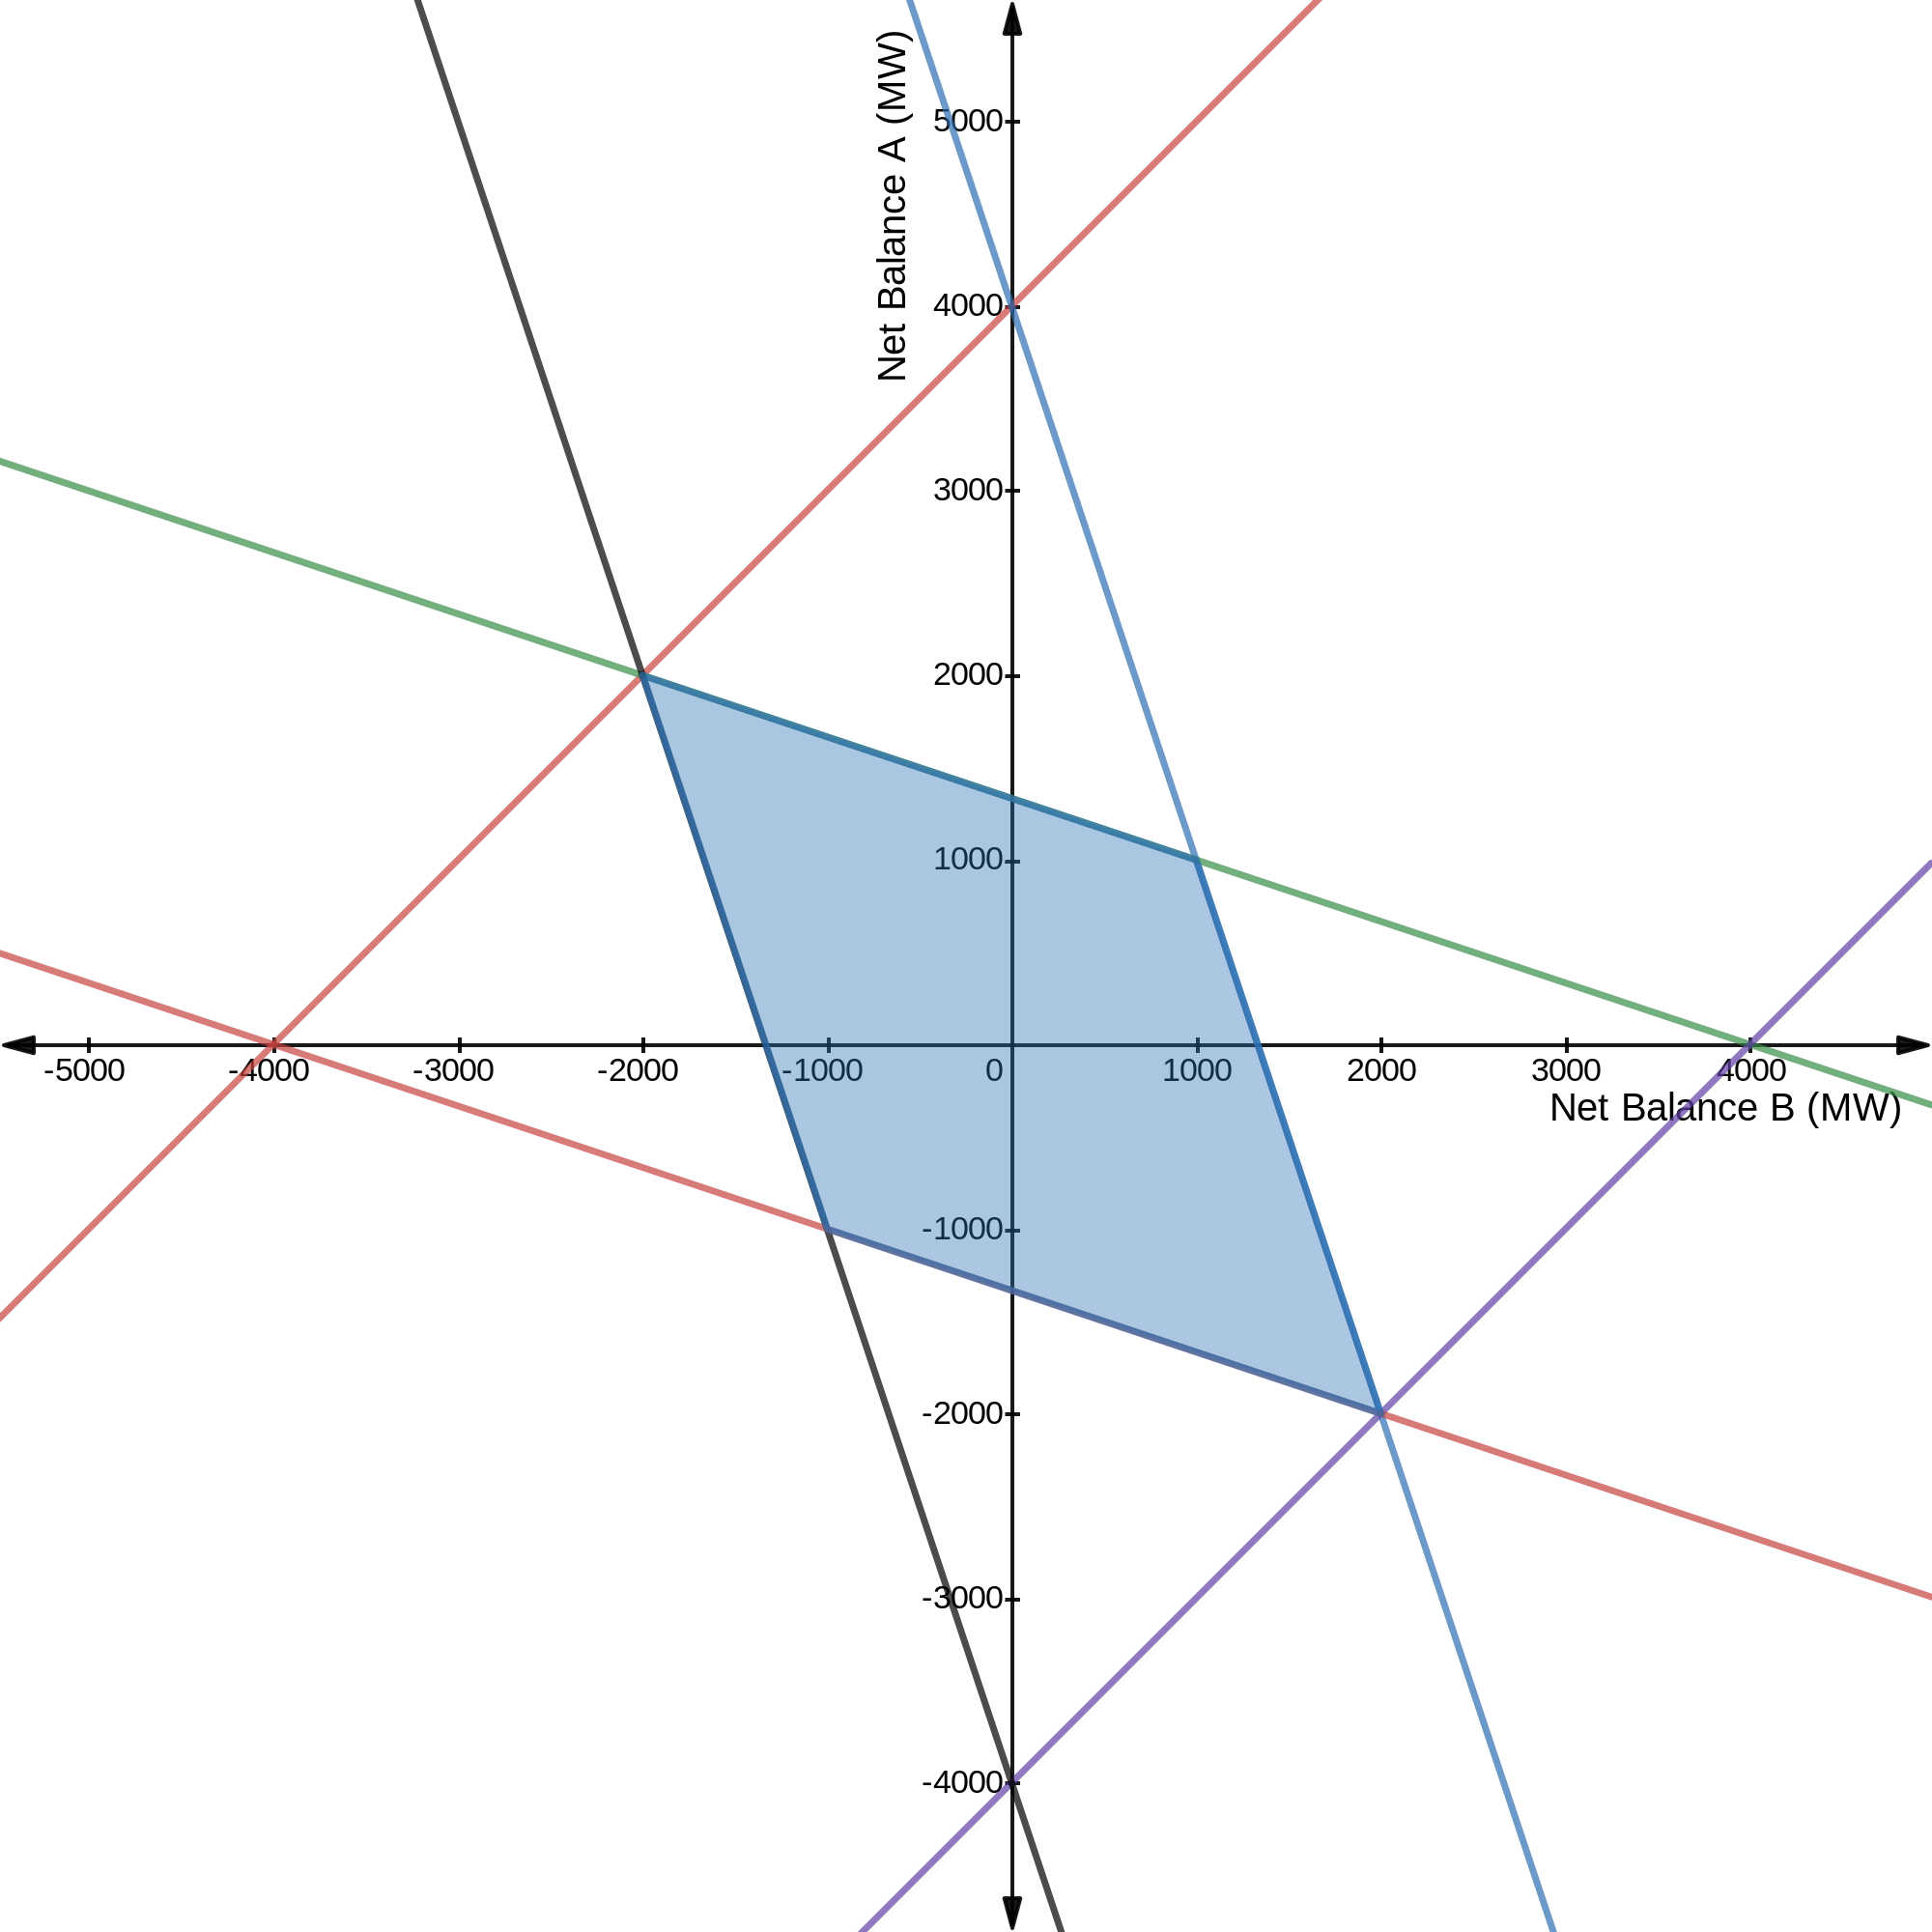
\includegraphics[width=0.6 \linewidth]{PTDF.png}
        \caption{FlowBased Domain}
        \label{fig:PTDF}
\end{figure}

The lines formed by the constraints form a certain feasible and bounded region. The domain is convex as the region is closed and finite. 

\section*{\textbf{Exercise 3}}

\begin{enumerate}
    \item \textbf{Maximum export positions feasible for Zone A, B and C}:
    \begin{itemize}
        \item Zone A
        \begin{itemize}
            \item When Zone A only exports without import: In this case, the maximum feasible export position is 1333.333 MW. The impedence between A and C in line 1 is 3R and line 2 is R. If the power were to flow through the line 2, the export will then have to be 4000 MW, which isn’t possible for the network. Therefore the power flow from line 1 is 1000MW/0.75 = 1333.33 MW.
            \item When Zone A and B export the power export is 1000 MW. Hence the maximum export is 1333.33 MW.
        \end{itemize}
        \item Zone B: The first quadrant is where both net balances are positive and hence in this quadrant is where the export can be analysed. Both the points (0,1333.3) and(1333.33,0) are corner points to this export area. Hence the maximum export position is 1333.33 MW
        \item Zone C: We have assumed that C acts as a slack bus and therefore the maximum export out of C is 0 MW
    \end{itemize}
    \item \textbf{Maximum bilateral exchange possible from Zone A to Zone B}: The points of consideration are the (±2000, ±2000) points from the figure \ref{fig:PTDF} where the net exchange of power is maximum. The maximum bilateral exchange from zone A to zone B is 2000, where the flow through each of the lines is 1000 MW.
    \item \textbf{In which situation is the line A-B the constraining line?}: The line A-B acts as a intersection point for the feasible region. It is evident that the A-B line does not act as constraining line if the line is moved further away from the feasible region. If the line A-B is moved into the feasible region it will act as a constraining line. 
    \item \textbf{Power flows between the different zones}:
    The below figure helps  determine the power flow between the different zones. Using this, it can also be verified the flow through any of the lines does not exceed the rating of the line, that is 1000 MW.

    \begin{figure}[H]
    \centering
        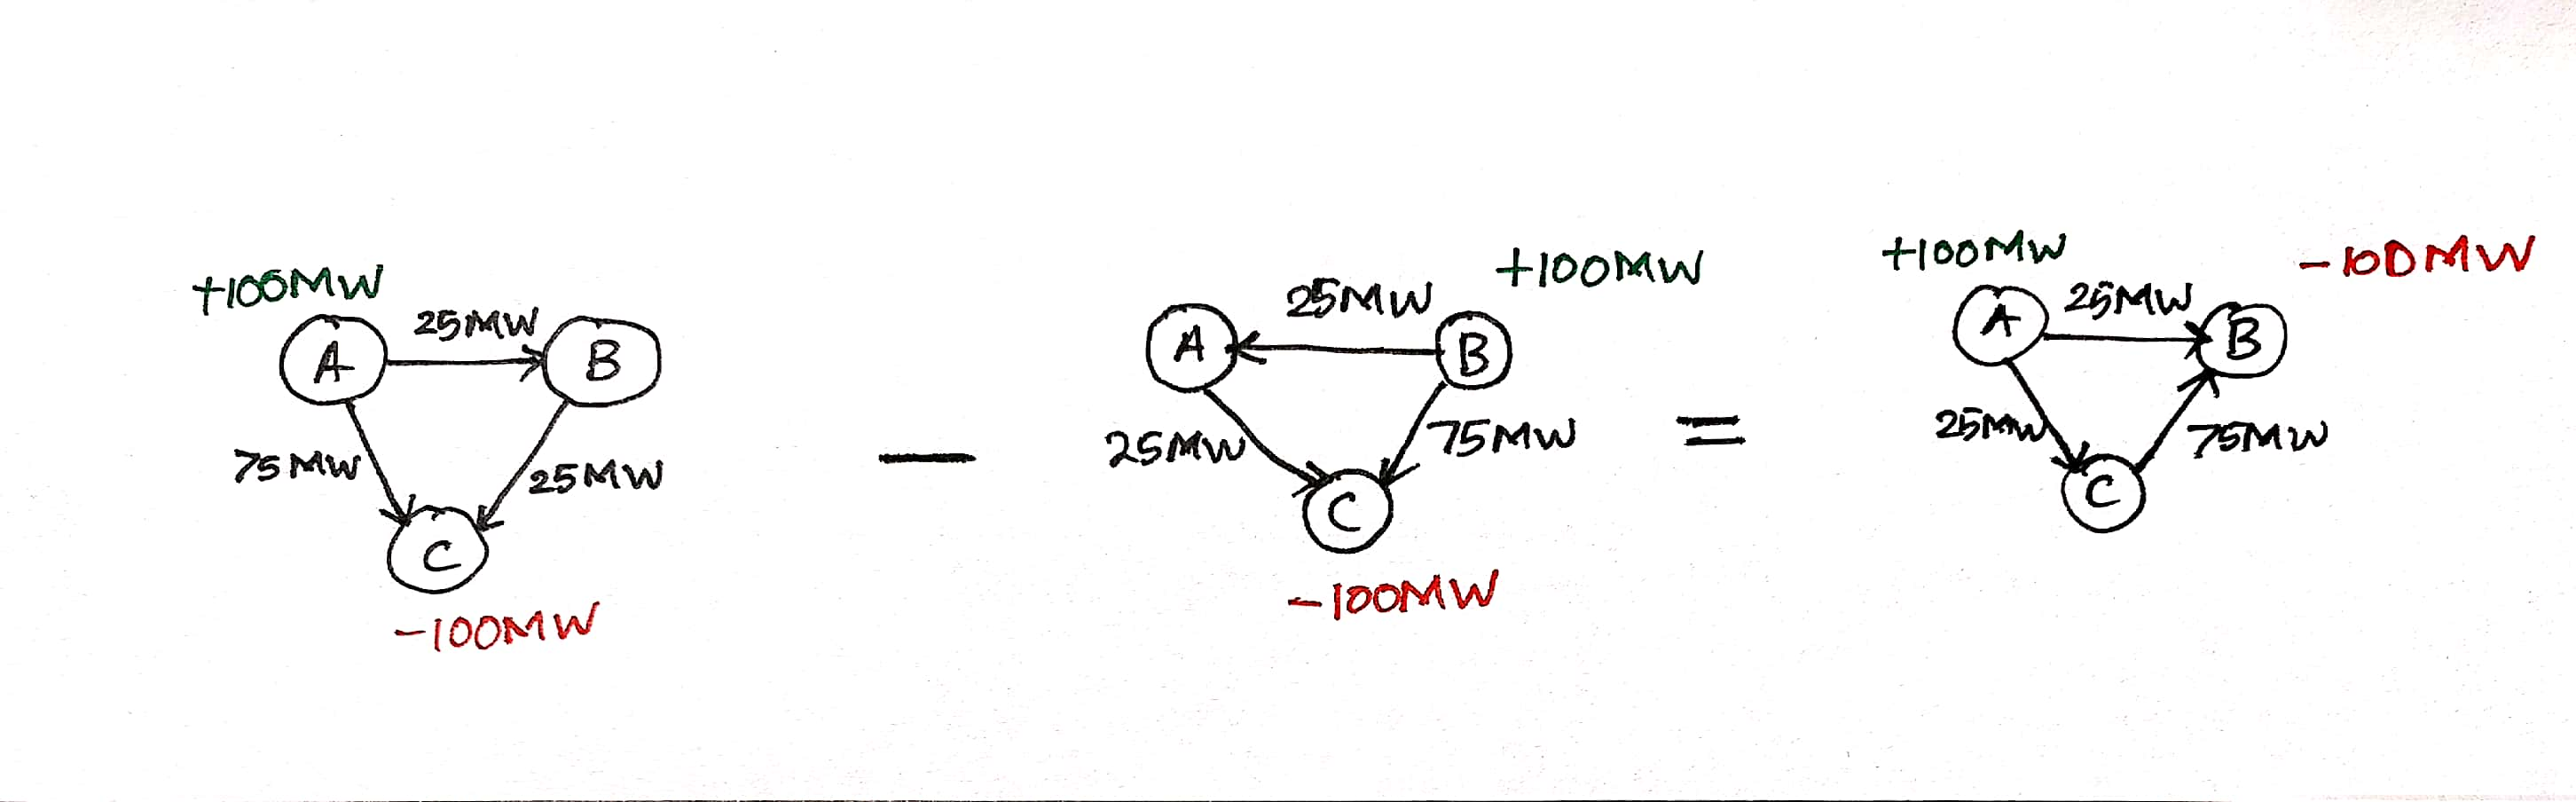
\includegraphics[width=1 \linewidth]{power_flow.jpg}
        \caption{Superposition used to determine flow}
        \label{fig:pf}
\end{figure}

\end{enumerate}

\section*{\textbf{Exercise 4}}

\textbf{Determine the net position shift for all zones needed to shift from the situation described in the previous exercise (max bilateral exchange from zone A to zone B) to the situation with a max bilateral exchange from zone B to zone A.
}

\[NP_ref = (-2000,2000)\]
\[NP_i = (2000,-2000)\]
\[F_ref = (-2000,2000)\]
\[PTDF = \pm 0.25\]

\begin{equation}
    F_i = F_ref + PTDF(NP_i - NP_ref) = (2000,-2000)
    \label{eq:equ1}
\end{equation}

With the given values of the parameters and using equation \ref{eq:equ1}, Fi is calculated as (2000,-2000). Therefore, net position shift for zone B is +4000, and net position shift for zone A is -4000 for the new exercise which is max bilateral exchange from zone B to A.
\newline

\textbf{Determine the flow on the line C-A in case of a maximum bilateral exchange from zone B to zone A by using the PTDF matrix to shift the FlowBased domain. }\\
1000 MW will flow through C-A. Since the impedance from node B to node A and the impedance from node B to node A via node C is equal.
